\documentclass{article}
\usepackage{polski} %może wymagac dokonfigurowania latexa, ale jest lepszy niż standardowy babel'owy [polish]
\usepackage[polish]{babel}
\usepackage[utf8]{inputenc}
\usepackage[OT4]{fontenc}
\usepackage{amsfonts}
\usepackage{graphicx,color} %include pdf's (and png's for raster graphics... avoid raster graphics!)
\usepackage{url}
\usepackage{here}
\usepackage[pdftex,hyperfootnotes=false,pdfborder={0 0 0}]{hyperref} %za wszystkimi pakietami; pdfborder nie wszedzie tak samo zaimplementowane bo specyfikacja nieprecyzyjna; pod miktex'em po prostu nie widac wtedy ramek
\usepackage[section]{placeins}

% Zmiana rozmiarów strony tekstu
\addtolength{\voffset}{-1cm}
\addtolength{\hoffset}{-1cm}
\addtolength{\textwidth}{2cm}
\addtolength{\textheight}{2cm}

%bardziej zyciowe parametry sterujace rozmieszczeniem rysunkow
\renewcommand{\topfraction}{.85}
\renewcommand{\bottomfraction}{.7}
\renewcommand{\textfraction}{.15}
\renewcommand{\floatpagefraction}{.66}
\renewcommand{\dbltopfraction}{.66}
\renewcommand{\dblfloatpagefraction}{.66}

\newcommand{\termdef}[1]{\emph{#1}}
\newcommand{\acronym}[1]{\emph{\MakeUppercase{#1}}}

\newcommand{\definicja}[1]{\termdef{#1}}
\newcommand{\akronim}[1]{\acronym{#1}}
\newcommand{\english}[1]{ang.~\emph{#1}}

\setcounter{topnumber}{9}
\setcounter{bottomnumber}{9}
\setcounter{totalnumber}{20}
\setcounter{dbltopnumber}{9}

% własny bullet list z malymi odstepami
\newenvironment{tightlist}{
\begin{itemize}
  \setlength{\itemsep}{1pt}
  \setlength{\parskip}{0pt}
  \setlength{\parsep}{0pt}}
{\end{itemize}}




\begin{document}

\thispagestyle{empty} %bez numeru strony

\begin{center}
{\large{Sprawozdanie z eksperymentu z przedmiotu\\
Metaheurystyki i Obliczenia Inspirowane Biologicznie}}

\vspace{3ex}



\vspace{3ex}
{\footnotesize\today}

\end{center}

\vspace{10ex}

Prowadzący: dr inż. Maciej Komosiński

\vspace{5ex}

Autorzy:
\begin{tabular}{lllr}
\textbf{Tomasz Ziętkiewicz} & inf84914 & ISWD & tomek.zietkiewicz@gmail.com \\
\end{tabular}

\vspace{5ex}

Zajęcia poniedziałkowe, 15:10.

\newpage



\begin{abstract}
Użycie klasyfikatora \emph{SVM} wymaga doboru odpowiedniej do danego problemu funkcji jądrowej. Jej wybór nie jest zadaniem trywialnym i może decydować o sprawności klasyfikatora. Postanowiono zbadać możliwość użycia programowania genetycznego w celu wygenerowania optymalnych funkcji jądrowych. Z użyciem biblioteki \emph{ECJ} stworzono algorytm programowania genetycznego, który generował poprawne funkcje jądrowe. Wartość ich przystosowania była sprawdzana za pomocą biblioteki \emph{LibSVM}.
Wyniki pokazują, że w przypadku pewnych zbiorów danych optymalizacja funkcji jądrowej ma znaczący wpływ na trafność klasyfikacji. Optymalne wyniki uzyskiwano już dla przebiegu trwającego jedną generację co sugeruje możliwość dalszej optymalizacji algorytmu.
\end{abstract}


\section{Wstęp}
	\subsection{Opis eksperymentu}
	Celem eksperymentu było użycie programowania genetycznego do wyewoluowania optymalnych funkcji jądrowych dla klasyfikatora \emph{SVM}.

	Klasyfikator SVM dokonuje klasyfikacji binarnej oddzielając od siebie dwie grupy przykładów hiperpłaszczyzną przebiegającą w przestrzeni atrybutów opisujących przykłady. Najczęściej grupy te nie są liniowo separowalne i trzeba dokonać transformacji cech opisujących przykłady do przestrzeni o większej liczbie wymiarów tak, żeby były w niej liniowo separowalne. Funkcje używane do dokonania tej transformacji to funkcje jądrowe  (inczej kernele  - ang. kernel functions). Wybór odpowiedniej funkcji zależy od rozwiązywanego problemu i zazwyczaj opiera się na doświadczeniu osoby używającej klasyfikator, posiadanej przez nią wiedzy dziedzinowej. W przypadku nie znanych \textit{apriori} danych wejściowych i braku doświadczenia w wyborze optymalnej funkcji jądrowej można posłużyć się automatycznymi metodami optymalizacji. Wśród nich idalną do tego zadania wydaje się \definicja{programowanie geetyczne} (\akronim{GP} - \english{Genetic Programming}). Jest to szczególny rodzaj \definicja{obliczeń ewolucyjnych} (\akronim{EC} - \english{Evolutionary Computing}), w którym ewoluowane osobniki to funkcje reprezentowane za pomocą struktur drzewiastych.
	
	Na potrzeby eksperymentu zaprojektowano algorytm programowania genetycznego, który ewoluował funkcje jądrowe poprzez łączenie ze sobą prostych funkcji jądrowych w funkcje złożone za pomocą funkcji łączących.
	Co ważne taki sposób generowania funkcji jądrowych zapewnia, że będą one poprawnymi funkcjami jądrowymi \cite{Shawe-Taylor:2004:KMP:975545}. Jest to własność domknięcia (\english{closure}) zbioru funkcji jądrowych ze względu na pewne operacje (funkcje łączące).

\subsection{Opis algorytmu}
	Przebieg algorytmu jest typowy dla algorytmów genetycznych:
\begin{enumerate}
\item Utwórz początkową populację kerneli
\item \label{ewaluacja} Oblicz wartość \textit{funkcji dopasowania} każdego z kerneli: dokładność klasyfikacji SVM z użyciem tego kernela
\item Jeśli znaleziono idealny kernel (dokładność klasyfikacji 100 ) lub skończył się czas, użyj tego kernela do klasyfikacji zbioru walidującego, zwróć wyniki klasyfikacji i zakończ algorytm.
\item Dokonaj selekcji najlepszych funkcji z populacji
\item Utwórz nową populację poprzez mutację i krzyżowanie wybranych w poprzednim kroku funkcji
\item Wróć do punktu \ref{ewaluacja}
\end{enumerate}

\begin{figure}[ht]
\centering
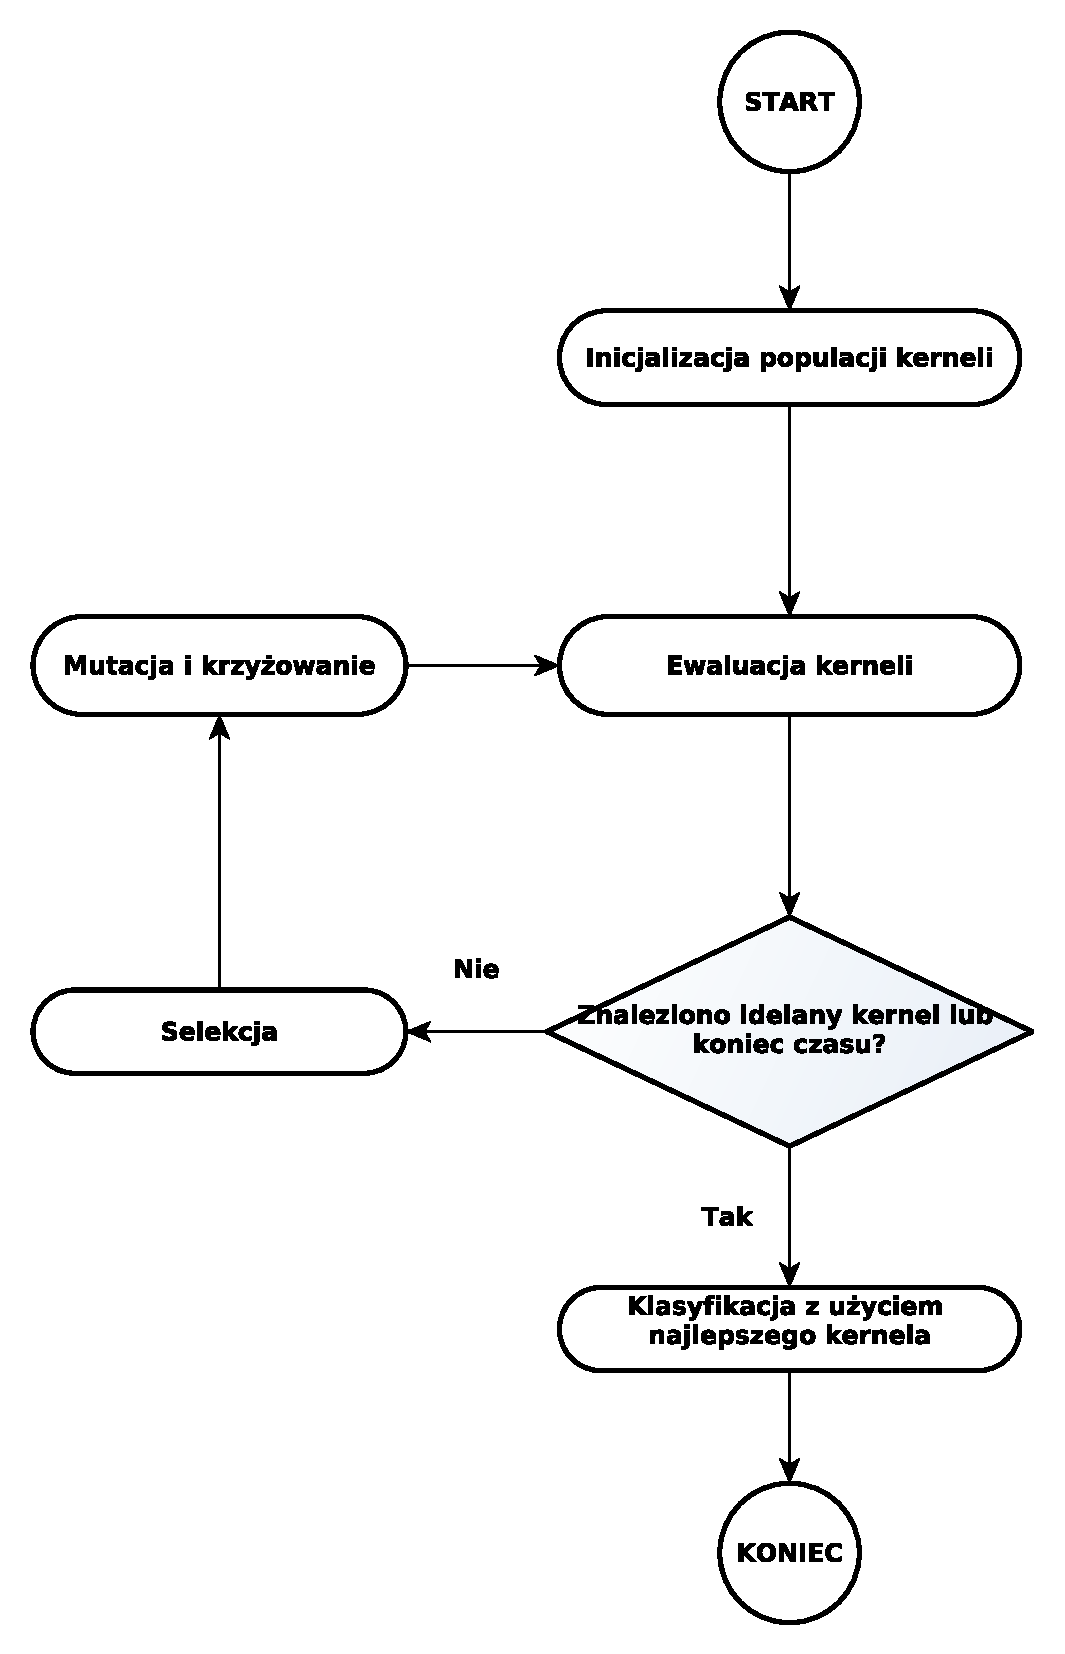
\includegraphics[scale=0.5]{figures/algorithm}
\caption{Diagram przepływu algorytmu Kernel GP.\label{fig:algorithm}}
\end{figure}

Algorytm pokazano również na diagramie przepływu na rycinie \ref{fig:algorithm}. 
Poszczególne kroki algorytmu zostaną opisane poniżej.

\subsection{Inicjalizacja populacji}
Podczas inicjalizacji początkowo pusta populacja jest zapełniana przez generowane w sposób losowy drzewa reprezentujące funkcje. Generowane drzewa muszą być poprawne, czyli spełniać narzucone ograniczenia na głębokość drzewa, liczbę węzłów, typ wartości zwracanych przez drzewo.
Wielkość populacji jest jednym z parametrów algorytmu. Zbyt mała populacja powoduje losowe zawężenie przeszukiwanej przestrzeni i zmniejsza prawdopodobieństwo znalezienia optymalnej funkcji. Z drugiej strony zbyt duża wielkość populacji upodabnia algorytm genetyczny do pełnego przeszukiwania, co oczywiście zwiększa szanse znalezienia optymalnego kernela, ale wydłuża czas działania algorytmu.

\subsubsection{Generowanie funkcji}
Generowanie drzew reprezentujących funkcje jądrowe polega na łączeniu ze sobą funkcji elementarnych zgodnie z  przypisanymi im ograniczeniami.
Funkcje elementarne wraz z ograniczeniami zdefiniowane w algorytmie:
\begin{itemize}
\item Funkcje łączące - jako argument przyjmują wynik dwóch lub jednej funkcji jądrowej i ewentualnie stałą \emph{ERC}. Zwracają wartość rzeczywistą. Dzięki właściwości domknięcia zbioru kerneli ze względu na operacje wykonywane przez te funkcje funkcja powstała przez połączenie dwóch kerneli funkcją łączącą jest również poprawnym kernelem \cite{Shawe-Taylor:2004:KMP:975545}.
	\begin{itemize}
	\item Dodawanie: $ k(x, z) = k_1(x,z) + k_2(x,z) $
	\item Mnożenie: $ k(x, z) = k_1(x,z) * k_2(x,z) $	
	\item Mnożenie przez stałą: $ k(x, z) = a * k_1(x,z) $
	\item Funkcja wykładnicza: $ k(x, z) = e ^{k_1(x,z)} $
	\end{itemize}
	Gdzie $ a $ to stała rzeczywista generowana jako stała \emph{ERC}.
\item Podstawowe funkcje jądrowe - jako argument przyjmują odpowiednią do funkcji liczbę stałych ERC. Zwracają wartość rzeczywistą.
	\begin{itemize}
	\item Liniowa: $ k(x, z) = \langle x,z \rangle $	
	\item Wielomianowa: $ k(x, z) = \langle x,z \rangle ^d $
	\item Gausowska: $ e^{-\gamma*||x-z||^2} $	
	\item Sigmoidalna: $ k(x, z) = \tanh(\gamma \langle x,z \rangle + \tau) $
	\end{itemize}
	Gdzie $ \gamma $, $ \tau $ oraz $ d $ to wartości stałe generowane jako stałe \emph{ERC}. a $ \langle x,y \rangle $ to iloczyn skalarny wektorów $x$ i $y$.
\item Stałe \akronim{ERC} (\english{Ephemeral Random Constant}) liczby rzeczywiste lub całkowite, które służą jako parametry innych funkcji. Są one liściami w drzewie, nie przyjmują żadnych argumentów. Mogą losowo zmieniać swoją wartość podczas mutacji.
	\begin{itemize}
	\item $ \gamma $: liczba rzeczywista z zakresu
	\item $ \tau $: liczba rzeczywista z zakresu
	\item $ d $: liczba całkowita z zakresu
	\item $ a $: liczba rzeczywista z zakresu
	\end{itemize}
\end{itemize}
Przykładowe drzewo wygenerowane przez algorytm pokazana na ryc.\ref{fig:tree}.

Wektory cech będące najważniejszymi argumentami funkcji jądrowych nie są wyodrębnione jako osobne węzły budujące drzewo, ponieważ są one danymi wejściowymi ewoluowanych funkcji i dla każdej ewoluowanej funkcji są takie same.		

\begin{figure}[ht]
\centering
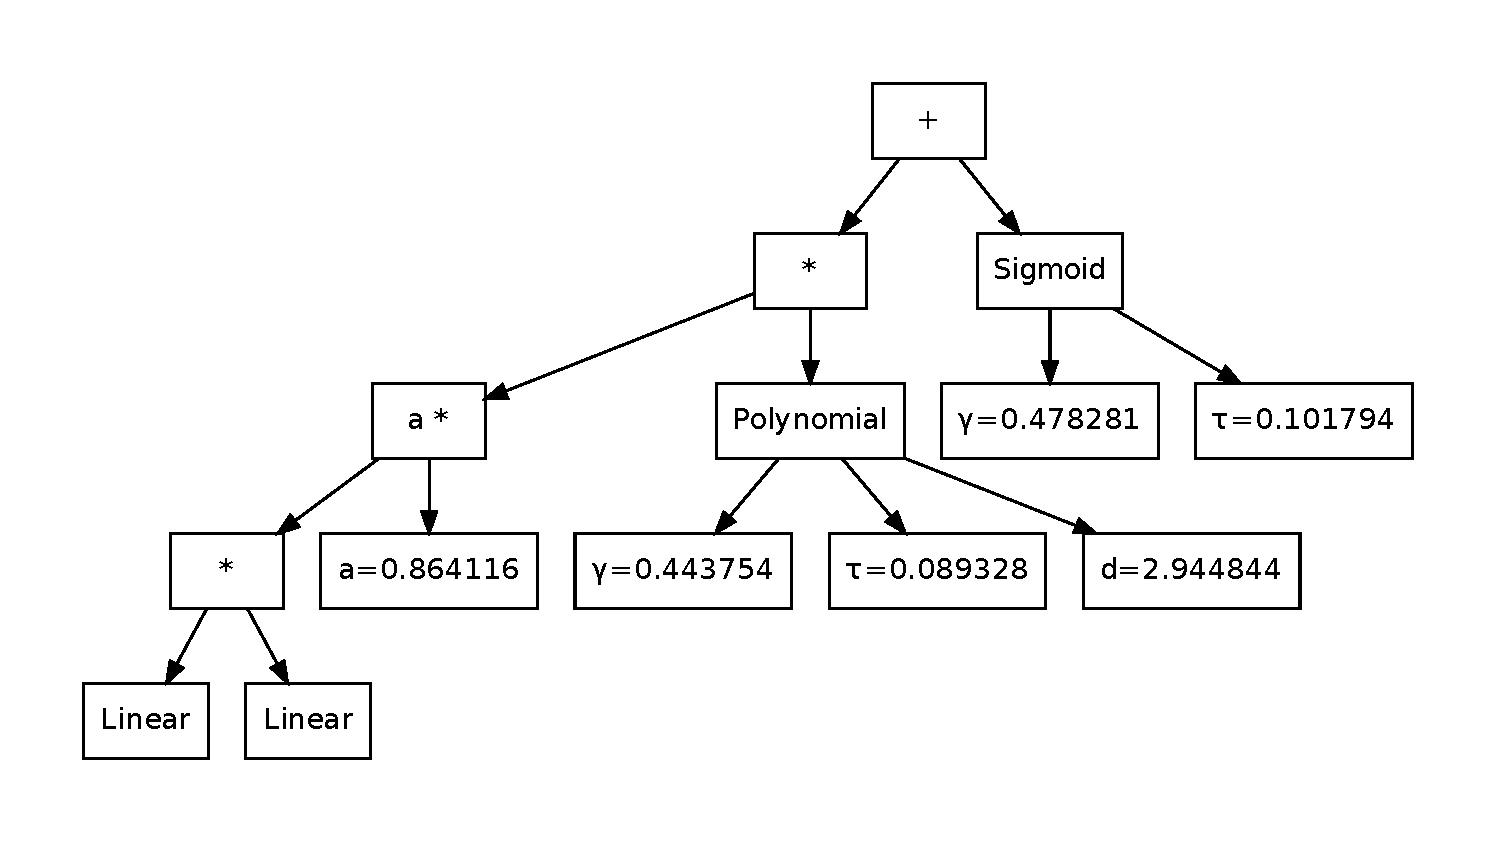
\includegraphics[scale=0.5]{figures/tree}
\caption{Przykładowe drzewo generowane przez algorytm.\label{fig:tree}}
\end{figure}


\subsection{Ewaluacja kerneli}
Ewaluacja funkcji jądrowej polega na jej zastosowaniu w algorytmie SVM do klasyfikacji zbioru testowego.
Otrzymana trafność stanowi miarę przystosowania (\english{fitness}) danej funkcji.

\subsection{Selekcja}
Jednym z problemów programowania genetycznego jest to, że drzewa powstałe w wyniku procesu ewolucyjnego mogą być bardzo duże, co nie jest pożądaną cechą - większe drzewo dłużej oblicza zwracaną wartość, zajmuje więcej miejsc w pamięci. Dlatego wielkość drzew należy ograniczać, jeśli wzrost drzewa nie prowadzi do zwiększenia wartości funkcji dopasowania.
Wielkość generowanych drzew jest regulowana przez dwa mechanizmy. Pierwszy to proste ograniczenie na maksymalną głębokość drzewa. Wartość tę ustawiono na 6 - drzewa o większej głebokości nie zostaną w ogóle wygenerowane przez podczas inicajlizacji populacji czy podczas krzyżowania i mutacji. Drugi mechanizm, o angielskiej nazwie \textit{parsimony pressure},  promuje mniejsze drzewa podczas selekcji. W tym celu stosowany jest algorytm selekcji turniejowej leksykograficznej z koszykami (ang. Bucket Lexicographic
 Tournament Selection). Algorytm ten sortuje populację według przystosowania osobników, następnie grupuje je w N "koszyki". Następnie selekcja przebiega według zasad selekcji turniejowej, z tym, że porównuje się nie przystosowanie osobników, ale koszyk, do którego są przypisane. W przypadku gdy w turnieju porównywane są dwa osobniki z tego samego koszyka wygrywa ten, który jest mniejszy.

\subsection{Krzyżowanie i mutacja}
Krzyżowanie polega na odcięciu dwóch losowych poddrzew z dwóch różnych osobników i zamianie ich miejscami. Wygenerowane w ten sposób drzewo musi spełniać narzucone na drzewo ograniczenia dotyczące typów i wielkości.
Mutacja drzew polega na zamianie losowo wybranego poddrzewa przez losowo wygenerowane drzewo.
Dodatkowo mutowane są również węzły ERC. Ich mutacja polega na dodaniu losowej wartości o rozkładzie normalnym do wartości przechowywanej w węźle. Wartość ta może być ujemna lub dodatnia.
Mutacji podlega $ 90\% $ drzew, pozostałe $ 10\% $ jest pozostawiane bez zmian. Wszystkie drzewa podlegające mutacji mają mutowane węzły ERC. Ponadto $ 70\% $ z nich podlega krzyżowaniu, $ 20\% $ mutacji polegającej na generowaniu losowych poddrzew a $ 10\% $ ma mutowane jedynie węzły ERC.

\subsection{Walidacja rozwiązania}
Walidacja polega na użyciu najlepszego znalezionego kernela do klasyfikacji przykładów ze zbioru walidującego, który nie był używany podczas uczenia klasyfikatora SVM ani podczas ewaluacji kerneli.
Najpierw algorytm SVM jest uczony na połączonych zbiorach trenującym i walidującym, przy pomocy tej funkcji jądrowej. Następnie dokonywana jest klasyfikacja zbioru walidującego. Otrzymana w wyniku tej klasyfikacji trafność jest miarą oceny całego algorytmu Kernel GP.

\section{Implementacja}
Algorytm został napisany w języku Java z użyciem bibliotek \textit{ECJ (Evolutionary Computing in Java)} \cite{sean_ecj_2010} oraz LibSVM \cite{chang_libsvm:_2011}. Pierwsza z nich dostarcza mechanizmy \textit{obliczeń ewolucyjnych} w tym \textit{programowania genetycznego}.
\emph{LibSVM} to klasyfikator SVM napisany oryginalnie w języku C z dostępną implementacją w Javie.
Mechanizmy \emph{ECJ} stanowią trzon algorytmu zapewniając tworzenie populacji funkcji, ich selekcję, mutację oraz krzyżowanie. \emph{LibSVM} został użyty na etapie ewaluacji wygenerowanych przez \emph{ECJ} funkcji.
	

\section{Wyniki}
	\subsection{Zbiory danych}
	Do oceny pracy algorytmu użyto standardowych zbiorów danych służących do testowania systemów maszynowego uczenia się, dostępnych na stronie biblioteki \emph{LIBSVM} \cite{chang_libsvm:_2011}. Zbiory zostały opisane w tabelce \ref{tab:datasets}.



\begin{table}[ht]
\begin{tabular}{||p{2cm}|c|p{1.5cm}|p{1.5cm}|p{1.5cm}|p{1.5cm}|p{1.5cm}||}
	\hline 
	Nazwa zbioru & Liczba klas & \hspace{0pt} Liczba atrybutów & \hspace{0pt} Wielkość zbioru uczącego & \hspace{0pt}Wielkość zbioru testującego & \hspace{0pt} Wielkość zbioru walidującego \\
	\hline 
	Iris & 3 & 4 & 68 & 33 & 49  \\ 
	\hline 
	Letter & 26 & 16 & 9000 & 4400 & 6600\\ 
	\hline 
	DNA & 3 & 180 & 1435 & 700 & 1051 \\ 
	\hline 
	Vowel & 11 & 10 & 447 & 217 & 326 \\ 
	\hline
	\end{tabular} 	
	\caption{Zbiory danych użyte do testowania systemu.\label{tab:datasets}} 	
\end{table}
	
	\subsection{Metodologia pomiarów}
	Żeby oszacować trafność klasyfikacji osiąganą przez skonstruowany system konieczne było podzielenie zbioru danych na zbiór uczący i walidujący, a w przypadku algorytmu Kernel-GP również wydzielenie ze zbioru uczącego podzbioru testującego, używanego do obliczania miary przystosowania (fitness) podczas przebiegu algorytmu genetycznego. Ponieważ sposób podziału zbioru danych ma wpływ na osiąganą trafność klasyfikacji, dokonywano 5 takich podziałów a następnie wyciągano średnią oraz odchylenie standardowe z wyników otrzymanych dla tych podziałów. Ta procedura dotyczyła zarówno testowania algorytmu \emph{Kernel-GP} jak i porównawczych testów klasyfikatora SVM z biblioteki \emph{LibSVM}. Dla obu algorytmów stosowano te same podziały danych, przy czym w przypadku klasyfikatora \emph{LibSVM} nie dzielono zbioru uczącego na trenujący i testujący.
	
	Jeśli nie zaznaczono inaczej, w poniższym omówieniu wyników słowa "dokładność" lub "trafność" klasyfikacji odnoszą się do trafności klasyfikacji danych ze zbioru walidującego.
	
	Algorytm genetyczny jest w swej naturze stochastyczny, korzysta więc z funkcji generujących liczby pseudolosowe. Aby zapewnić powtarzalność wyników i umożliwić ich porównanie ziarno generatora liczb pseudolosowych ustawiono na stałą wartość.

	Aby ocenić skuteczność algorytmu genetycznego w poszukiwaniu optymalnych funkcji jądrowych oraz oszacować optymalną wielkość populacji oraz czas trwania (liczbę ewaluowanych generacji) algorytmu przeprowadzono szereg eksperymentów obliczeniowych, w których uruchamiano algorytm dla coraz to większych wartości tych parametrów. Dla każdego przebiegu algorytmu zapisywano trafność klasyfikacji zbioru walidującego.

	Analizując tak zebrane dane można przeanalizować na ile poszukiwanie funkcji jądrowej przez algorytm genetyczny było podobne do losowego przeszukiwania a na ile było ono zbieżne. W pierwszym przypadku na wyniki osiągane przez algorytm powinna mieć wpływ przede wszystkim wielkość populacji, w drugim również liczba generacji przez które poszukiwano rozwiązania. W szczególności ciekawym przypadkiem jest ten, gdy liczba generacji wynosi 1, czyli cały algorytm ogranicza się do wygenerowania populacji losowych osobników i wybrania jednego z nich - w tym przypadku algorytm genetyczny sprowadza się do losowego poszukiwania rozwiązania. Porównując różnicę w trafności osiąganej w trakcie jednej generacji i coraz większej ich liczby można ocenić czy proces ewolucyjny przebiega poprawnie. 
	

	\subsection{Trafność klasyfikacji\label{sec:trafnosc}}
	Jak widać na rysunkach \ref{fig:acc-iris}-\ref{fig:acc-letter-detailed} sprawność algorytmu zależy mocno od konkretnego zbioru danych. Na przykład zbiór IRIS jest na tyle łatwy w klasyfikacji, że ciężko jest poprzez dobranie optymalnej funkcji jądrowej polepszyć znacznie wyniki klasyfikacji.
	Na osiąganą trafność klasyfikacji wpływ ma też podział zbioru danych na testujący, uczący i walidujący - widać to po odchyleniu standardowym widocznym na wykresach.
	
	\subsubsection{Monotoniczność funkcji trafności}
	
	Miejscami funkcja trafności nie jest monotoniczna, a ściślej niemalejąca, względem liczby generacji oraz wielkości populacji (co widać np. na wykresach \ref{fig:acc-iris-detailed} i \ref{fig:acc-vowel-detailed}). Wydawałoby się, że tak być nie powinno (algorytm genetyczny zwraca najlepszego osobnika z całego swojego przebiegu, więc wszystkie osobniki, które pojawiły się podczas przebiegu z 5 generacjami pojawią się podczas przebiegu z 7 generacjami, więc trafność dla przebiegu z 7 generacjami powinna być co najmniej tak dobra jak dla przebiegu z 5 generacjami). Jednak może się tak zdarzyć ze względu na to, że trafność pokazana na wykresach to trafność klasyfikacji zbioru walidującego, natomiast trafność użyta przez algorytm genetyczny jako miara dostosowania (\english{fitness}) to trafność klasyfikacji zbioru testującego. Widać to na wykresie \ref{fig:fit-iris-detailed}, który przedstawia wartość przystosowania dla tych samych danych, dla których na wykresie \ref{fig:acc-iris-detailed} jest pokazana trafność klasyfikacji na zbiorze walidującym - tutaj funkcja wykazuje mniej braku monotoniczności. 
	
	Zatem przynajmniej część braku monotoniczności funkcji trafności na zbiorze walidującym wynika z przeuczenia algorytmu - znaleziona przez algorytm genetyczny funkcja jądrowa lepiej sprawdza się przy klasyfikacji zbioru testującego niż walidującego. Nie jest to jednak jedyna przyczyna braku monotoniczności - widać to na wykresie \ref{fig:fit-vowel-detailed} przedstawiającym wartość funkcji przystosowania dla zbioru \emph{vowel} - jej przebieg jest bardzo podobny do przebiegu ukazanej na rys. \ref{fig:acc-vowel-detailed} funkcji trafności klasyfikacji zbioru walidującego na tym samym zbiorze. Co więc jest przyczyną braku monotoniczności? Warto zauważyć, że funkcja jest niemalejąca ze względu na ilość generacji oraz że dla jednej generacji funkcja jest monotoniczna. Sugeruje to, że "winnym" może być selekcja - w praktyce nie zachodzi ono w przypadku gdy algorytm genetyczny działa przez jedną generację.
    
    \begin{figure}[H]
		
\includegraphics[scale=0.50]{figures/functions/func1}
		\caption{Funkcja z pierwszej generacji, która w przebiego z wielkością populacji 4 osiągnęła fitness $0.4242424$. Przodek funkcji z rys.\ref{fig:func2} \label{fig:func1}}
	\end{figure}
	
	\begin{figure}[H]
		
\includegraphics[scale=0.60]{figures/functions/func2}
		\caption{Funkcja z trzeciej generacji, która w przebiego z wielkością populacji 4 osiągnęła fitness $0.78030306$. Potomek funkcji z rys.\ref{fig:func1}, przodek zwycięskiej funkcji (rys.\ref{fig:func5}) z przebiegu z populacją o wielkości 4.\label{fig:func2}}
	\end{figure}
          
   	\begin{figure}[H]
		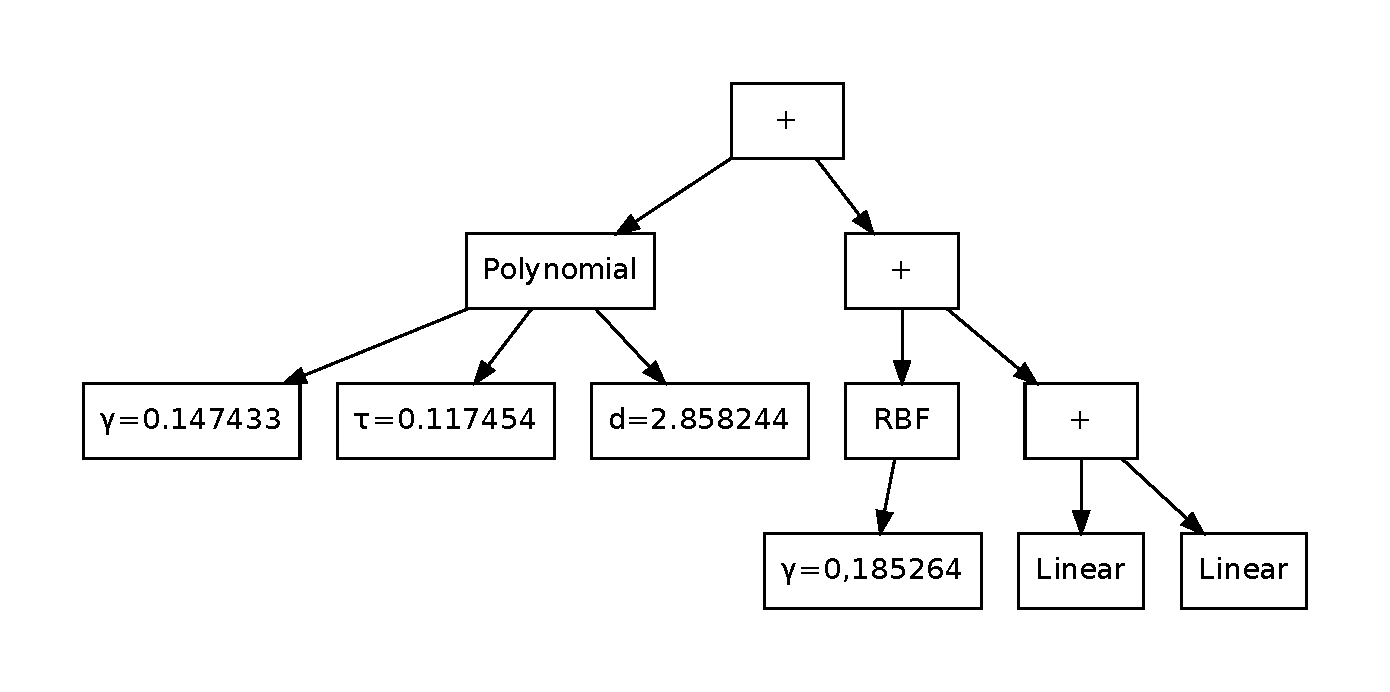
\includegraphics[scale=0.60]{figures/functions/func5}
		\caption{Funkcja z ostatniej generacji w przebiegu z wielkością populacji 4 osiągnęła fitness $0.8333333$. Przodek zwycięskiej funkcji z rys.\ref{fig:func4} \label{fig:func5}}
	\end{figure}          


   	\begin{figure}[H]
		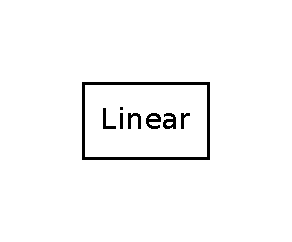
\includegraphics[scale=0.60]{figures/functions/func3}
		\caption{Funkcja z trzeciej generacji, która w przebiegu z wielkością populacji 3 i 4 osiągnęła fitness $0.6515151$. Przodek zwycięskiej funkcji z rys.\ref{fig:func4}\label{fig:func3}}
	\end{figure}                 

    	\begin{figure}[H]
		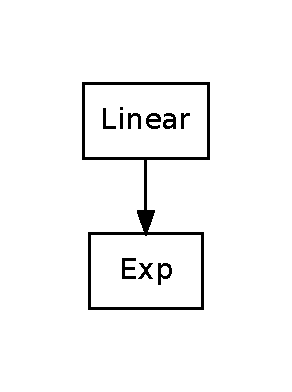
\includegraphics[scale=0.60]{figures/functions/func4}
		\caption{Zwycięska funkcja w przebiegu z populacją wielkości 3, potomek funkcji z rys.\ref{fig:func3}. Osiągnęła fitness $0.9015151$. \label{fig:func4}}
	\end{figure} 	
	
	 Gdy przyjrzeć się dokładnie przebiegowi ewolucji widać, że rzeczywiści tak jest. Dodatkowy osobnik (rys. \ref{fig:func1}), który odróżnia w generacji pierwszej populacje o wielkości 3 i 4 jest przodkiem innego osobnika (rys. \ref{fig:func2}), który w trzeciej generacji osiąga fitness większy niż osobnik (rys. \ref{fig:func3}), który w przypadku populacji wielkości 3 był przodkiem osobnika (rys. \ref{fig:func4}), który to okazał się najlepszym podczas przebiegu całego algorytmu. W rezultacie tego "geny" potencjalnego zwycięzcy nie przetrwały w przebiegu algorytmu z populacją liczącą 4 osobników. Jak widać osobnik najlepszy we wszystkich generacjach nie musi być wcale potomkiem osobników najlepszych w poszczególnych generacjach - czasem połączenie dwóch osobników przeciętnych może dać osobnika bardzo dobrego. 	
	
	\begin{figure}[ht]
		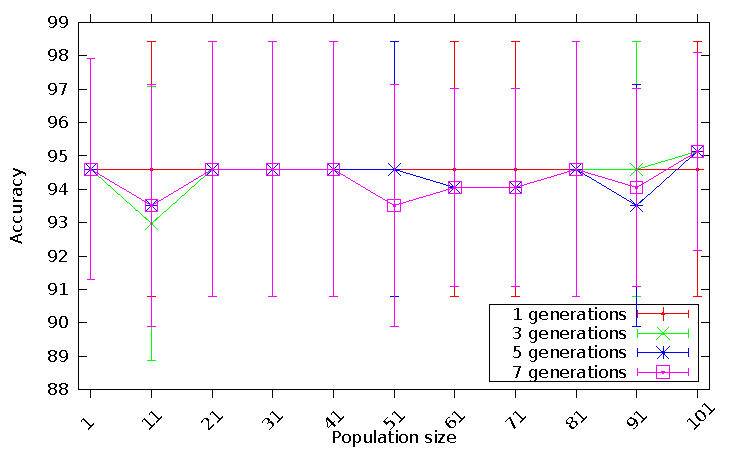
\includegraphics[scale=0.90]{figures/accuracy-iris}
		\caption{Dokładność klasyfikacji dla zbioru \emph{iris} w funkcji rozmiaru populacji dla róznych ilości generacji.\label{fig:acc-iris}}
	\end{figure}
	
	\begin{figure}[ht]
		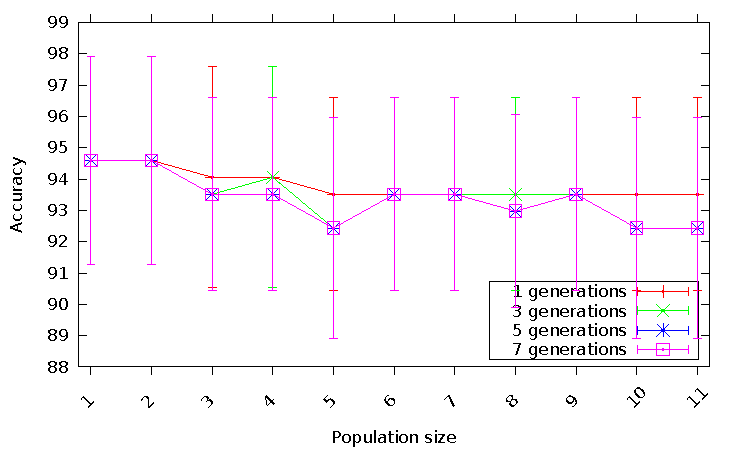
\includegraphics[scale=0.90]{figures/accuracy-iris-detailed}
		\caption{Dokładność klasyfikacji dla zbioru \emph{iris} w funkcji rozmiaru populacji dla róznych ilości generacji, dla małych populacji.	\label{fig:acc-iris-detailed}}
	\end{figure}	
	
	
		\begin{figure}[ht]
		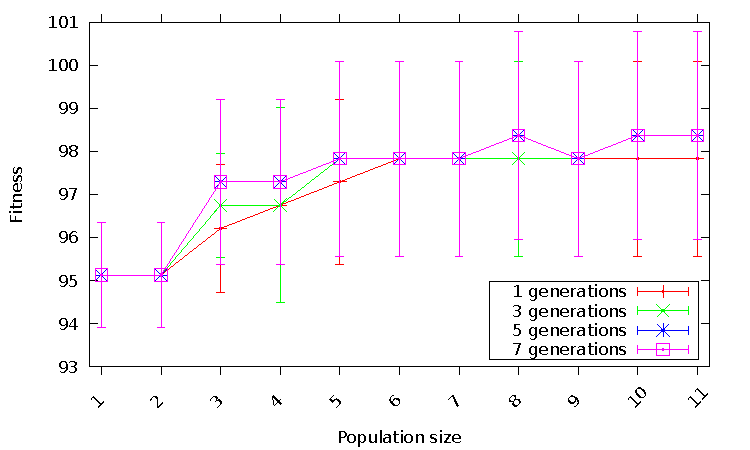
\includegraphics[scale=0.90]{figures/fitness-iris-detailed}
		\caption{Najlepsza wartość funkcji przystosowania (\english{fitness})  \emph{iris} w funkcji rozmiaru populacji dla róznych ilości generacji, dla małych populacji.	\label{fig:fit-iris-detailed}}
	\end{figure}	
	
		\begin{figure}[ht]
		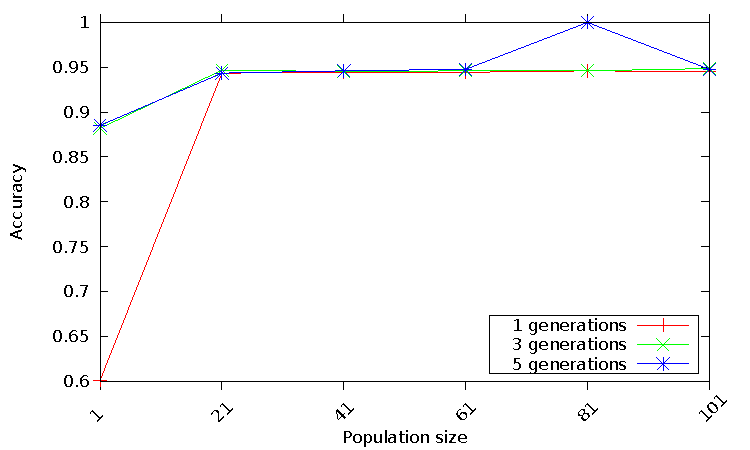
\includegraphics[scale=0.90]{figures/accuracy-dna}
		\caption{Dokładność klasyfikacji dla zbioru \emph{DNA} w funkcji rozmiaru populacji dla róznych ilości generacji.\label{fig:acc-dna}}
	\end{figure}
	
		\begin{figure}[ht]
		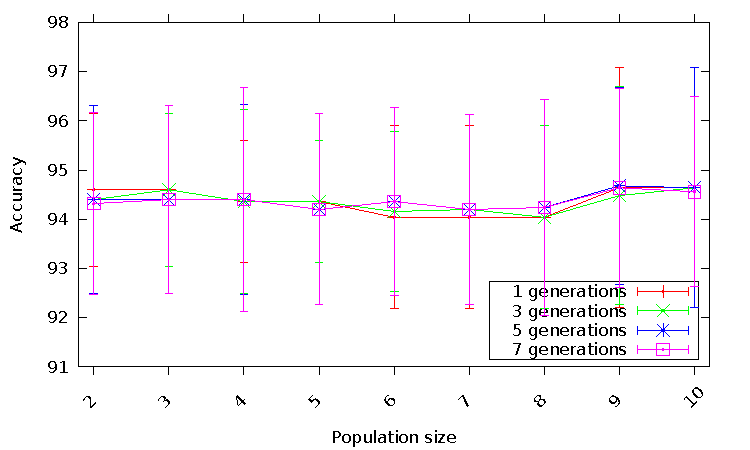
\includegraphics[scale=0.90]{figures/accuracy-dna-detailed}
		\caption{Dokładność klasyfikacji dla zbioru \emph{DNA} w funkcji rozmiaru populacji dla róznych ilości generacji, dla małych populacji.\label{fig:acc-dna-detailed}}
	\end{figure}	
	

		\begin{figure}[ht]
		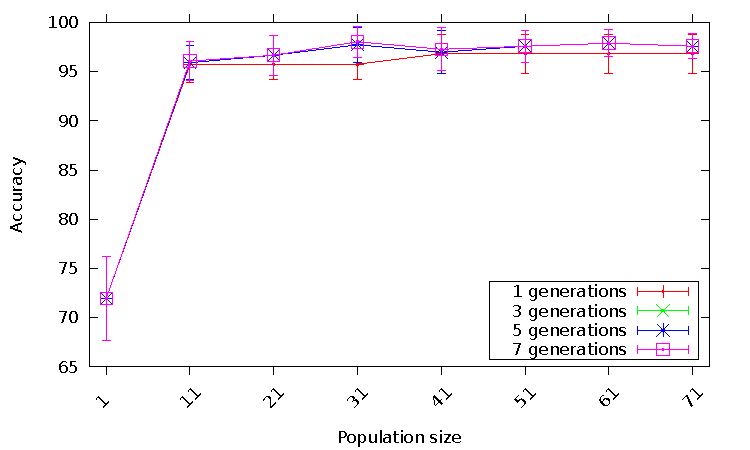
\includegraphics[scale=0.90]{figures/accuracy-vowel}
		\caption{Dokładność klasyfikacji dla zbioru \emph{vowel} w funkcji rozmiaru populacji dla róznych ilości generacji.\label{fig:acc-vowel}}
	\end{figure}
		
		\begin{figure}[ht]
		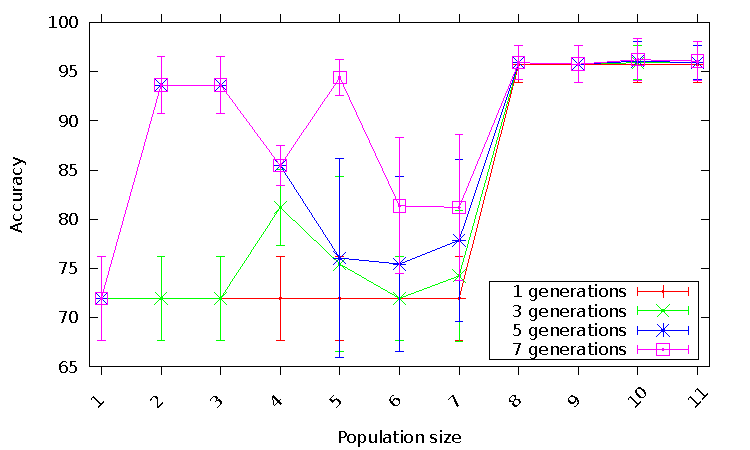
\includegraphics[scale=0.90]{figures/accuracy-vowel-detailed}
		\caption{Dokładność klasyfikacji dla zbioru \emph{vowel} w funkcji rozmiaru populacji dla róznych ilości generacji, dla małych populacji.\label{fig:acc-vowel-detailed}}
		\end{figure}
		
		\begin{figure}[ht]
		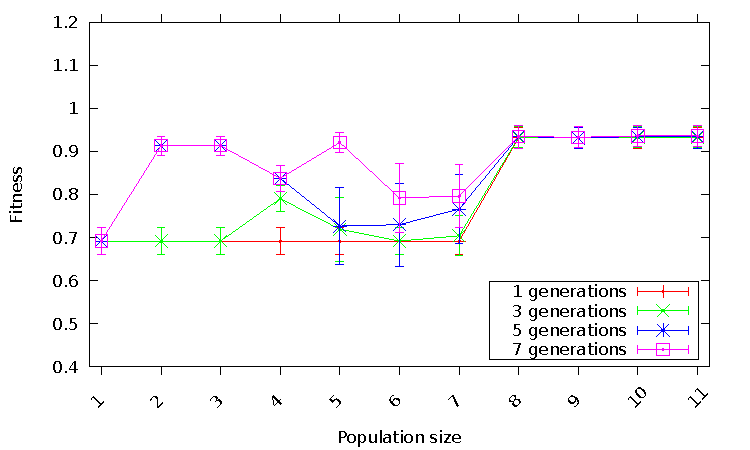
\includegraphics[scale=0.90]{figures/fitness-vowel-detailed}
		\caption{Dokładność klasyfikacji dla zbioru \emph{vowel} w funkcji rozmiaru populacji dla róznych ilości generacji, dla małych populacji.\label{fig:fit-vowel-detailed}}
		\end{figure}
	
	
		\begin{figure}[ht]
		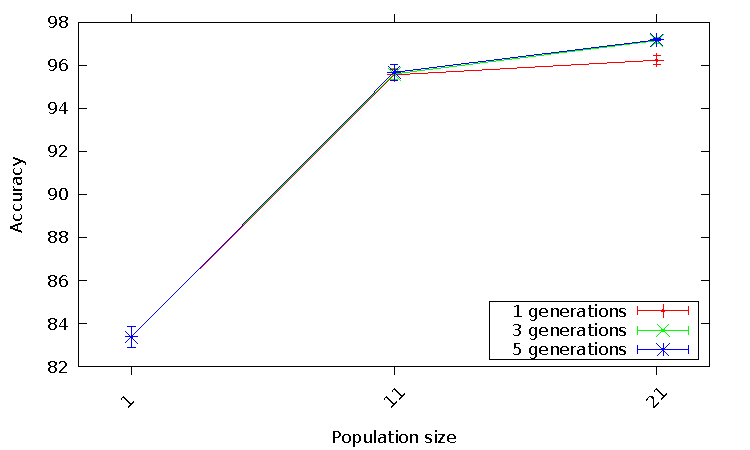
\includegraphics[scale=0.90]{figures/accuracy-letter}
		\caption{Dokładność klasyfikacji dla zbioru \emph{letter} w funkcji rozmiaru populacji dla róznych ilości generacji.\label{fig:acc-letter}}
	\end{figure}
		
				\begin{figure}[ht]
		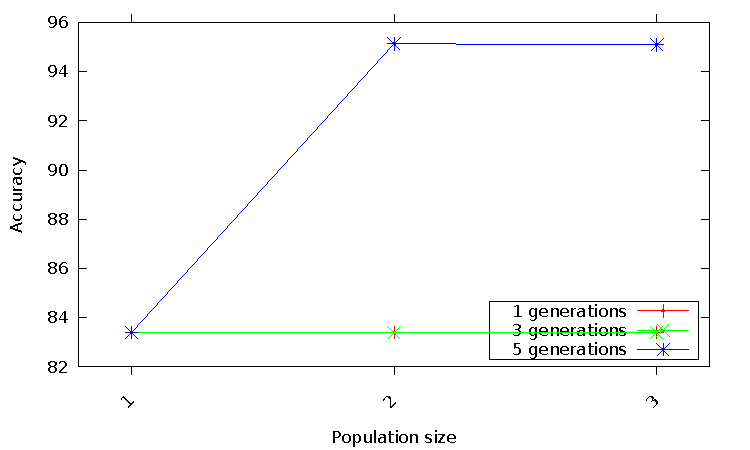
\includegraphics[scale=0.90]{figures/accuracy-letter-detailed}
		\caption{Dokładność klasyfikacji dla zbioru \emph{letter} w funkcji rozmiaru populacji dla róznych ilości generacji, dla małych populacji.\label{fig:acc-letter-detailed}}
	\end{figure}
		


	\subsection{Porównanie z tradycyjnym algorytmem SVM}
	Na wykresach \ref{fig:acc-iris-svm}-\ref{fig:acc-letter-svm} przedstawiono porównanie trafności klasyfikacji zbioru walidującego przez algorytm SVM z użyciem czterech podstawowych funkcji jądrowych (liniowej, wielomianowej, RBF i sigmoidalnej) i przez stworzony algorytm Kernel-GP.
	W przypadku dwóch zbiorów: \emph{vowel} i \emph{letter} udało się uzyskać polepszenie trafności klasyfikacji względem standardowych funkcji jądrowych. Są to zbiory, dla których standardoy SVM osiąga słabe wyniki - ok. $ 70%-80% $. 
	W przypadku dwóch pozostałych zbiorów niezależnie od użytej funkcji jądrowej osiągana trafność klasyfikacji jest bardzo wysoka - ok. $ 95% $ - sugeruje to, że zbiory te są dość łatwo separowalne z wyjątkiem $ 5% $ przypadków.
	
	\begin{figure}[ht]
		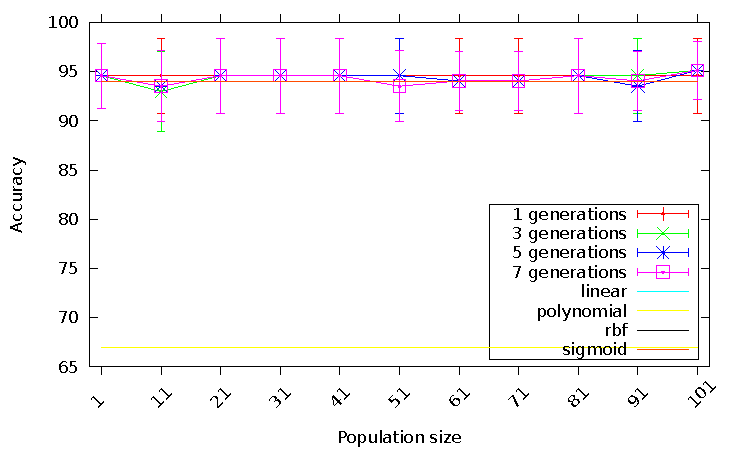
\includegraphics[scale=0.90]{figures/accuracy-iris-svm}
		\caption{Porównanie dokładności klasyfikacji dla zbioru \emph{iris} przez algorytm SVM z różnymi funkcjami jądrowymi i algorytm Kernel-GP\label{fig:acc-iris-svm}}
	\end{figure}
	
		\begin{figure}[ht]
		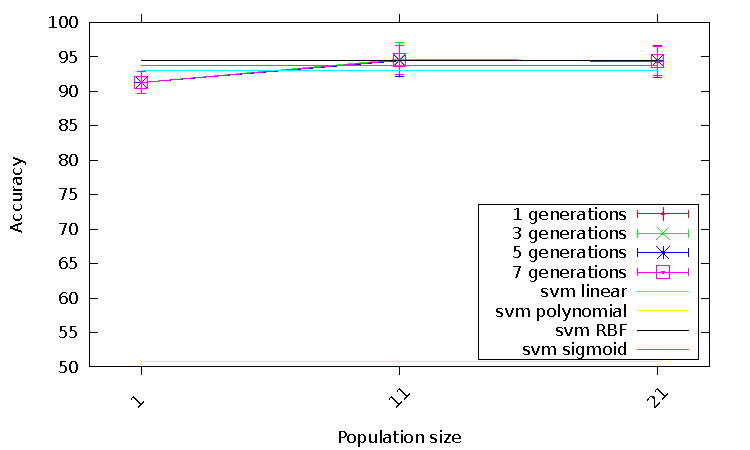
\includegraphics[scale=0.90]{figures/accuracy-dna-svm}
		\caption{Porównanie dokładności klasyfikacji dla zbioru \emph{dna} przez algorytm SVM z różnymi funkcjami jądrowymi i algorytm Kernel-GP.\label{fig:acc-dna-svm}}
	\end{figure}	
	
		\begin{figure}[ht]
		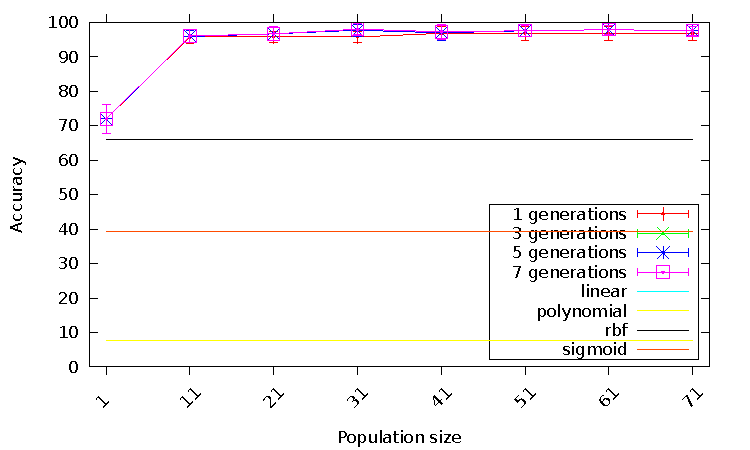
\includegraphics[scale=0.90]{figures/accuracy-vowel-svm}
		\caption{Porównanie dokładności klasyfikacji dla zbioru \emph{vowel} przez algorytm SVM z różnymi funkcjami jądrowymi i algorytm Kernel-GP\label{fig:acc-vowel-svm}}
	\end{figure}
	
		\begin{figure}[ht]
		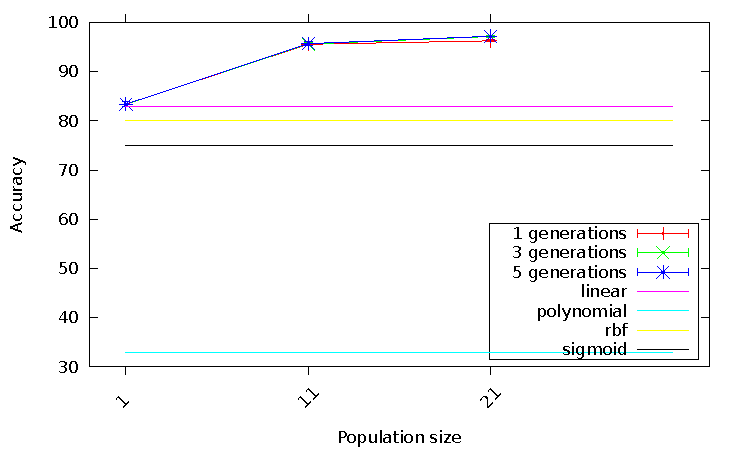
\includegraphics[scale=0.90]{figures/accuracy-letter-svm}
		\caption{Porównanie dokładności klasyfikacji dla zbioru \emph{letter} przez algorytm SVM z różnymi funkcjami jądrowymi i algorytm Kernel-GP\label{fig:acc-letter-svm}}
	\end{figure}		
		
		
\section{Podsumowanie}
	\subsection{Wnioski}
		Algorytm programowania genetycznego pozwala znaleźć optymalne funkcje jądrowe dla klasyfikatora SVM. W przypadku trudnych zbiorów różnice w trafności klasyfikacji mogą być znaczące. Kosztem jaki trzeba zapłacić za polepszenie jakości klasyfikacji jest czas obliczeń, który wzrasta wielokrotnie, choć należy pamiętać, że raz wyewoluowanej funkcji można używać wielokrotnie dla nowych danych.
		
		Rozważane w rozdziale \ref{sec:trafnosc} różnice między trafnością osiągana dla różnych czasów trwania algorytmu (ilości ewoluowanych generacji) są mało znaczące i widoczne tylko dla bardzo małych populacji. Dla większych populacji okazuje się, że wyniki są tak samo dobre dla jednej jak i dla wielu generacji. To niestety pokazuje, że algorytm programowania genetycznego w tym przypadku upodobnił się do losowego przeszukiwania - skoro przy odpowiednio dużej (nawet tak mało jak 4-8) wielkości populacji liczba generacji nie ma znaczenia dla osiąganego wyniku - nawet dla jednej generacji wyniki są takie same jak dla większej ich liczby - oznacza to, że mechanizm krzyżowania nie spełnia kluczowej roli w poszukiwaniu rozwiązań - wystarczy wygenerować odpowiednio dużą liczbę losowych funkcji jądrowych. Może być to spowodowane tym, że przeszukiwany krajobraz rozwiązań (funkcji jądrowych) jest dość jednolity, cechuje się małą zmiennością - choć przestrzeń rozwiązań jest bardzo duża, to są one zgrupowane w zbiory funkcji nie różniących się od siebie znacznie pod względem trafności klasyfikacji. Możliwe, że należałoby zmienić parametry procesu ewolucyjnego tak, żeby poszerzyć zakres generowanych funkcji, np. poluzować ograniczenie na głębokość funkcji. Mała liczba przebadanych zbiorów danych również może być przyczyną - możliwe, że dla innych zbiorów, mniej standardowych, które trudniej rozdzielić przy pomocy standardowych funkcji SVM, wyniki byłyby inne. Wreszcie można by poszerzyć zbiór funkcji bazowych, z których algorytm genetyczny generuje funkcje bardziej złożone - należałoby jednak zadbać o zachowanie ich poprawności.

%%%%%%%%%%%%%%%% literatura %%%%%%%%%%%%%%%%

\bibliography{bibliografia}
\bibliographystyle{plain}

\end{document}

